\section{Utilizzo SDK}
\begin{frame}
  \frametitle{Hello Bubble - How to}
  %[caption=My Javascript Example]
  \begin{center}
    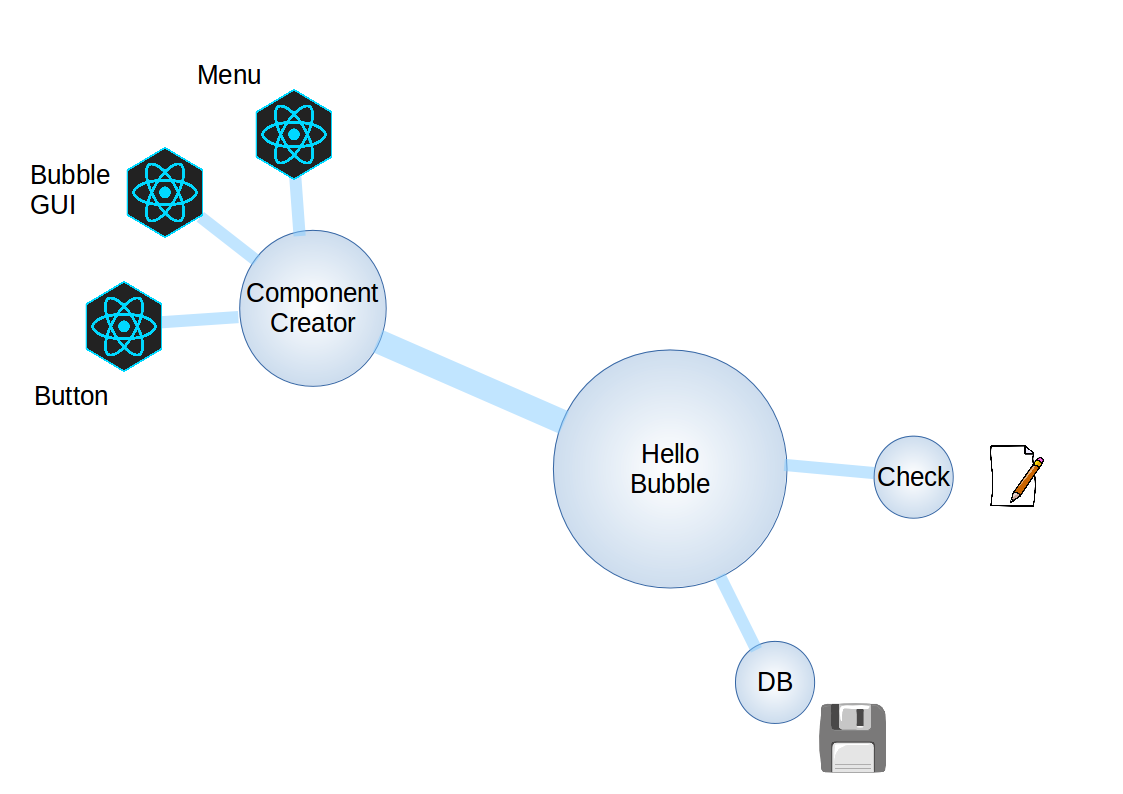
\includegraphics[scale=0.30]{code/bubbleMap.png}
  \end{center}
\end{frame}

\subsection{Hello Bubble - Gui}
\begin{frame}[fragile]
  \frametitle{Bubble Menu}
  %[caption=My Javascript Example]
  \begin{minipage}{.65\textwidth}
      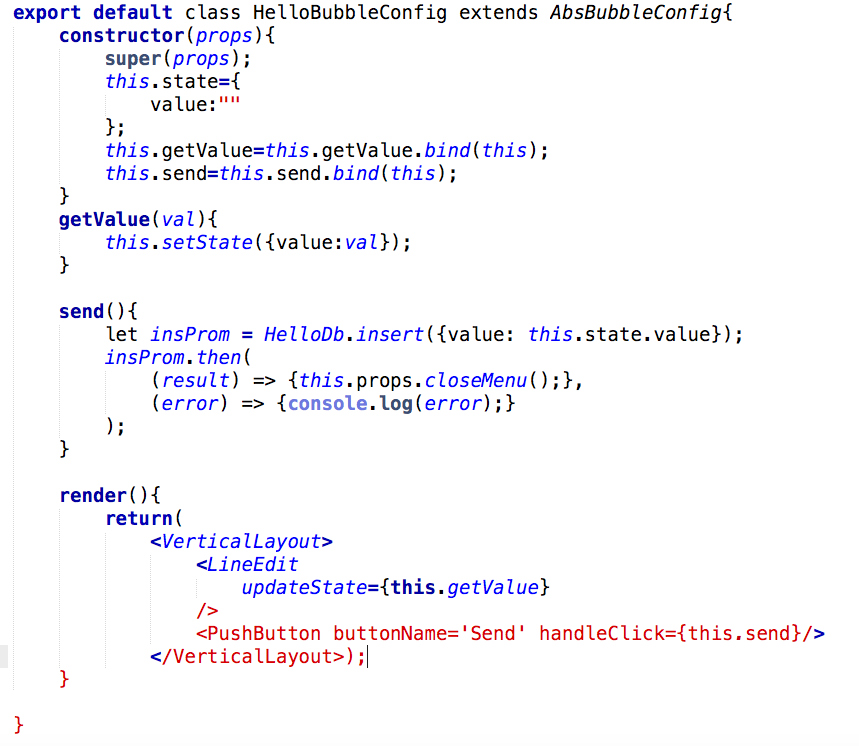
\includegraphics[width=\textwidth]{code/hellobubbleconfig.png}
  \end{minipage}
  \begin{minipage}{.34\textwidth}
      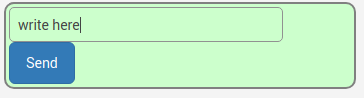
\includegraphics[width=\textwidth]{code/config.png}
  \end{minipage}
\end{frame}

\begin{frame}
  \frametitle{Bubble Button}
  %[caption=My Javascript Example]
  \begin{center}
  \begin{minipage}{.70\textwidth}
    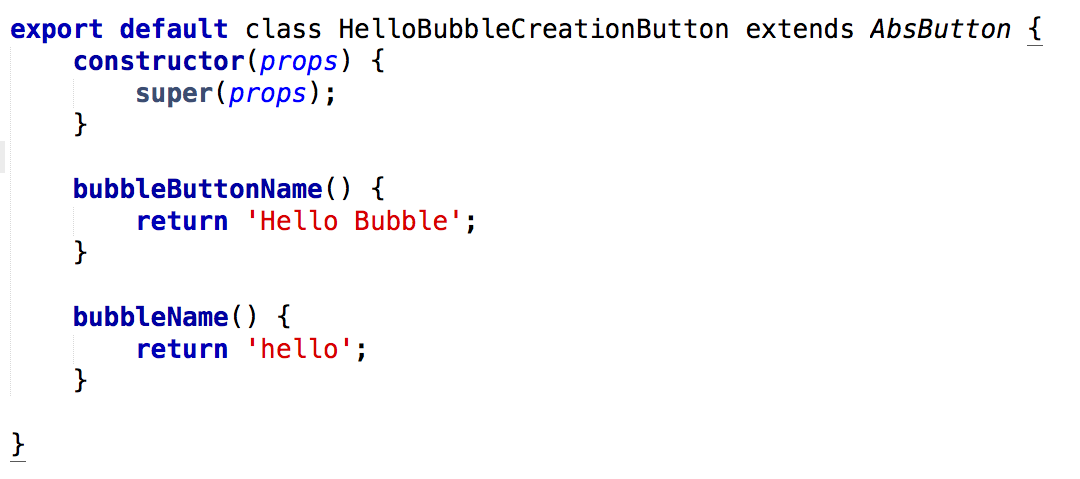
\includegraphics[width=\textwidth]{code/hellobubblecreationbutton.png}
  \end{minipage}
  \begin{minipage}{.28\textwidth}
    
\includegraphics[width=\textwidth]{code/button.png}
  \end{minipage}
  \end{center}
\end{frame}

\begin{frame}
  \frametitle{Bubble Gui}
  %[caption=My Javascript Example]
  \begin{center}
  \begin{minipage}{.65\textwidth}
    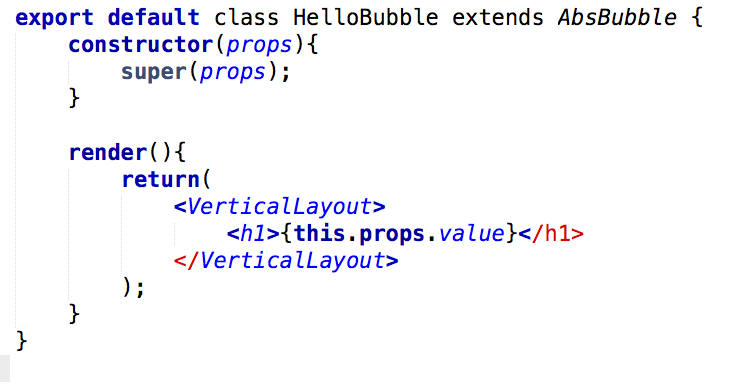
\includegraphics[width=\textwidth]{code/hellobubble.png}
  \end{minipage}
    \begin{minipage}{.34\textwidth}
    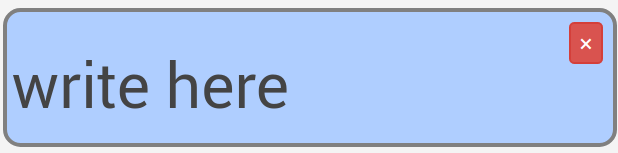
\includegraphics[width=\textwidth]{code/bubble.png}
  \end{minipage}
  \end{center}
\end{frame}


\begin{frame}
  \frametitle{Gui managment}
  %[caption=My Javascript Example]
  \begin{center}
    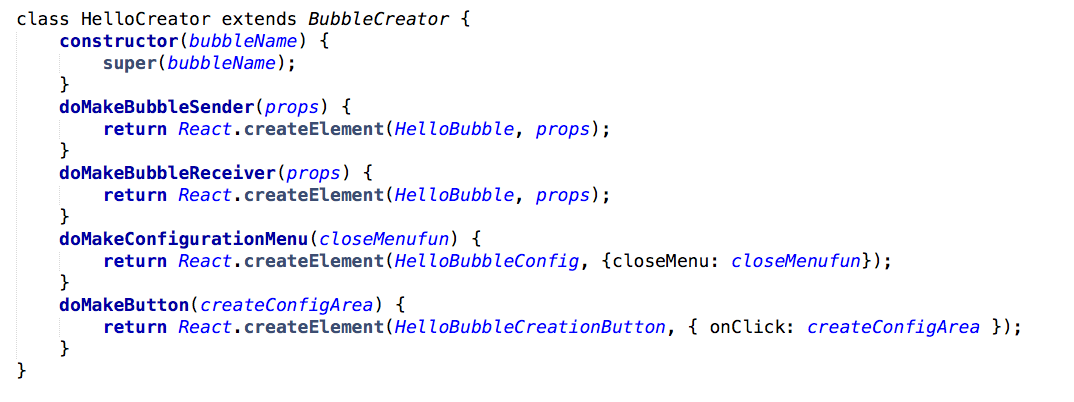
\includegraphics[width=.9\textwidth]{code/hellocreator.png}
  \end{center}
\end{frame}


\subsection{Database and data check}

\begin{frame}
  \frametitle{Database}
  %[caption=My Javascript Example]
  \begin{center}
    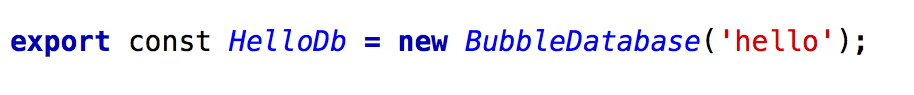
\includegraphics[width=.8\textwidth]{code/helloDb.png}
  \end{center}
\end{frame}

\begin{frame}
  \frametitle{Bubble Check}
  %[caption=My Javascript Example]
  \begin{center}
    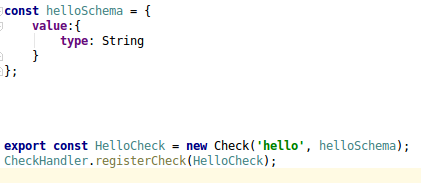
\includegraphics[width=.8\textwidth]{code/hellocheck.png}
  \end{center}
\end{frame}
